\documentclass[final,hyperref={pdfpagelabels=false}]{beamer}
\usepackage{grffile}
\mode<presentation>{\usepackage{../themes/beamerthemePersyval}}
\usepackage[english]{babel}
\usepackage[latin1, utf8]{inputenc}
\usepackage{amsmath,amsthm, amssymb, latexsym, mathabx}
%\usepackage{times}\usefonttheme{professionalfonts}  % obsolete
%\usefonttheme[onlymath]{serif}
\boldmath
\usepackage[orientation=portrait,size=a0,scale=1.4,debug]{beamerposter}
% change list indention level
% \setdefaultleftmargin{3em}{}{}{}{}{}

%\usepackage{snapshot} % will write a .dep file with all dependencies, allows for easy bundling

\usepackage{array,booktabs,tabularx}
\usepackage{wrapfig}
\newcolumntype{Z}{>{\centering\arraybackslash}X} % centered tabularx columns
%\newcommand{\pphantom}{\textcolor{ta3aluminium}} % phantom introduces a vertical space in p formatted table columns??!!

\listfiles

%%%%%%%%%%%%%%%%%%%%%%%%%%%%%%%%%%%%%%%%%%%%%%%%%%%%%%%%%%%%%%%%%%%%%%%%%%%%%%%%%%%%%%
\graphicspath{{../img/}}

\title{Eye-tracking and electroencephalogram data analysis using hidden semi-Markov models to identify reading strategies}
\author{Brice Olivier\textsuperscript{1,2}, Jean-Baptiste Durand\textsuperscript{1,2}, Anne Guérin-Dugué\textsuperscript{3}, Marianne Clausel\textsuperscript{2}}
\institute{\textsuperscript{1}Inria, \textsuperscript{2}Laboratoire Jean Kuntzmann, \textsuperscript{3}Gipsa-lab}
\date[June 13rd-14th, 2017]{June 13rd-14th, 2017}


%%%%%%%%%%%%%%%%%%%%%%%%%%%%%%%%%%%%%%%%%%%%%%%%%%%%%%%%%%%%%%%%%%%%%%%%%%%%%%%%%%%%%%
\newlength{\columnheight}
\setlength{\columnheight}{93cm}

%%%%%%%%%%%%%%%%%%%%%%%%%%%%%%%%%%%%%%%%%%%%%%%%%%%%%%%%%%%%%%%%%%%%%%%%%%%%%%%%%%%%%%
\begin{document}
\begin{frame}
    \begin{block}{Study purpose}
        \begin{columns}[T]
          \begin{column}{.50\paperwidth}
              \begin{itemize}
                  \item[\bullet] Textual information search is an unhomogeneous process in time (Simola, 2008)
                  \item[\drsh] Reading and decision processes are intertwined
              \end{itemize}
          \end{column}
          \begin{column}{.50\paperwidth}
              \begin{itemize}
                  \item[\bullet] Proposal : use a data-driven approach in order to separate these processes
                  \item[\bullet] Have the reading strategies contrasted characteristics in terms of EEGs?
              \end{itemize}
          \end{column}
        \end{columns}
    \end{block}

  \begin{columns}
    % ---------------------------------------------------------%
    % Set up a column
    \begin{column}{.50\textwidth}
      \begin{beamercolorbox}[center,wd=\textwidth]{postercolumn}
        \begin{minipage}[T]{.98\textwidth}  % tweaks the width, makes a new \textwidth
          \parbox[t][\columnheight]{\textwidth}{ % must be some better way to set the the height, width and textwidth simultaneously
            % Since all columns are the same length, it is all nice and tidy.  You have to get the height empirically
            % ---------------------------------------------------------%
            % fill each column with content
            \begin{block}{Experiment description}
                \begin{itemize}
                    \item[\bullet] 15 participants, 60 texts per participant
                    \item[\bullet] Presentation of a goal topic, e.g. in french "chasse aux oiseaux" (birds hunting), and a text, extracted from LeMonde, 1999
                    \item[\bullet] Question : is the text related to the topic ?
                \end{itemize}
                \begin{minipage}{0.47\textwidth}
                    \begin{figure}[h]
                        \centering
                        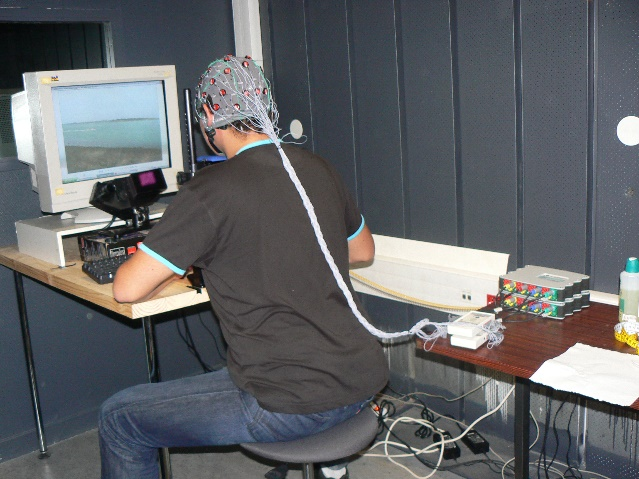
\includegraphics[width=18cm]{efrp.jpg}
                    \end{figure}
                \end{minipage} \hfill
                \begin{minipage}{0.47\textwidth}
                    \begin{figure}[h]
                        \centering
                        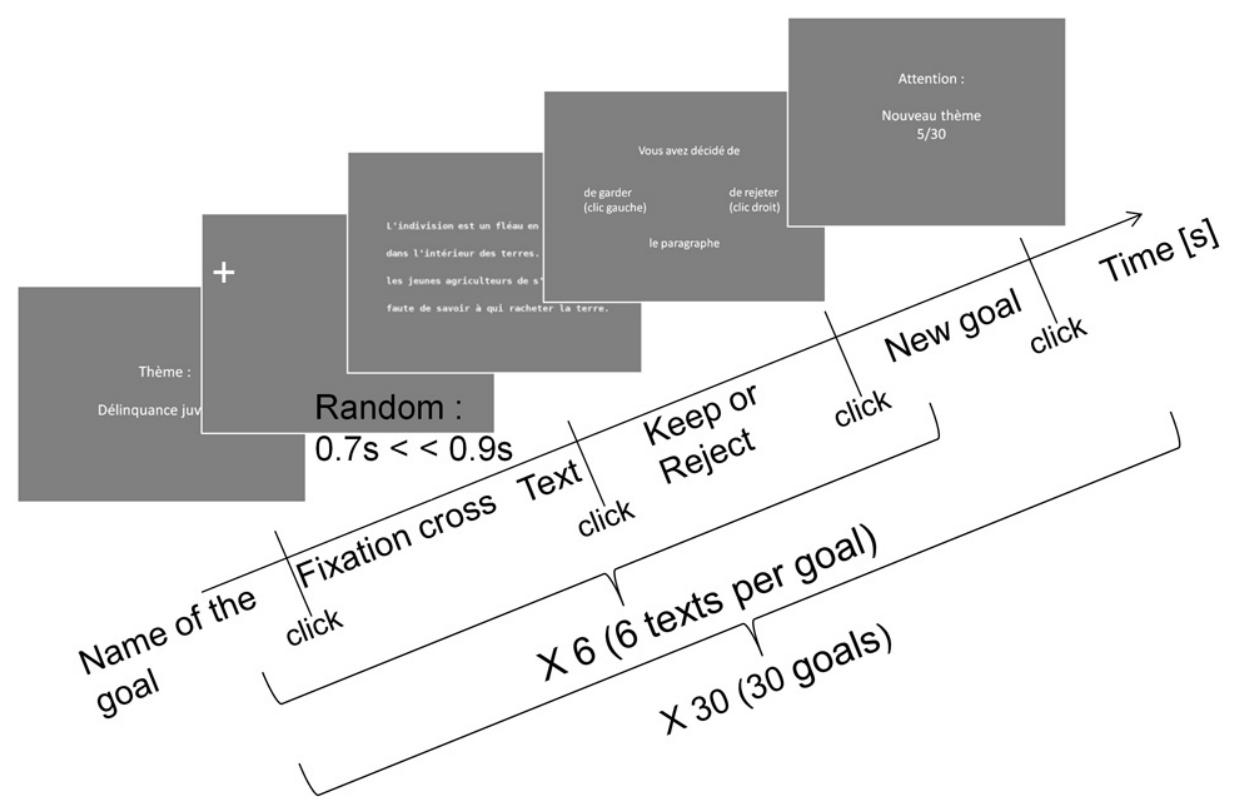
\includegraphics[width=18cm]{experiment_description.jpg}
                        \caption{Frey, 2013}
                    \end{figure}
                \end{minipage}
                \begin{itemize}
                    \item[\bullet] Measurements of eye positions over time and 30-channel EEG
                \end{itemize}
            \end{block}

            \vfill
            \begin{block}{Data pre-processing}
                \textbf{Raw data :} Participants, texts, coordinates X,Y of fixations at each time $t$.
                \vskip0.5cm
                \textbf{Data augmentation :}
                \begin{itemize}
                    \item[\bullet] Fixation duration, saccade amplitude
                    \item[\bullet]
                    \begin{minipage}{0.45\textwidth}
                        Word fixated
                    \end{minipage}
                    \begin{minipage}{0.35\textwidth}
                        \begin{figure}[H]
                            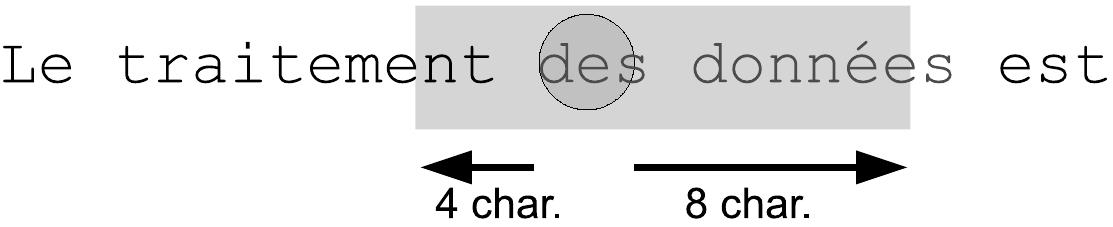
\includegraphics[width=1\linewidth]{fixation_window.jpg}
                            %\caption{Scanpath : alternance of fixations (circle, ratio proportional to duration) and saccades (lines).}
                        \end{figure}
                    \end{minipage}
                    \item[\bullet] Number of words between two fixations
                    \item[\bullet] Semantic proximity of the words in each text to the target topic (Latent Semantic Analysis + Cosine distance)
                \end{itemize}
                \vskip0.5cm
                \textbf{Observed process :} Readmode :  number of words between two fixations \{ $>$ 1, 1, 0, -1 , $<$ -1\}
                \vskip0.5cm
                \textbf{Model covariates :} Fixation duration, saccade amplitude, proximity of the fixated word to the topic

            \end{block}
            \vfill
            \begin{block}{Problems}
                \begin{itemize}
                    \item[\bullet] Identify reading strategies, obtain a segmentation of scanpaths with meaningful EEG interpretation
                    \item[\bullet] Change point detection model to catch changes of phase
                    \item[\bullet] The sojourn time using reading strategies should have relaxed hypothesis
                \end{itemize}
            \end{block}
            \vfill
            \begin{block}{Hidden semi-Markov models (Yu 2010)}
                \begin{figure}[H]
                    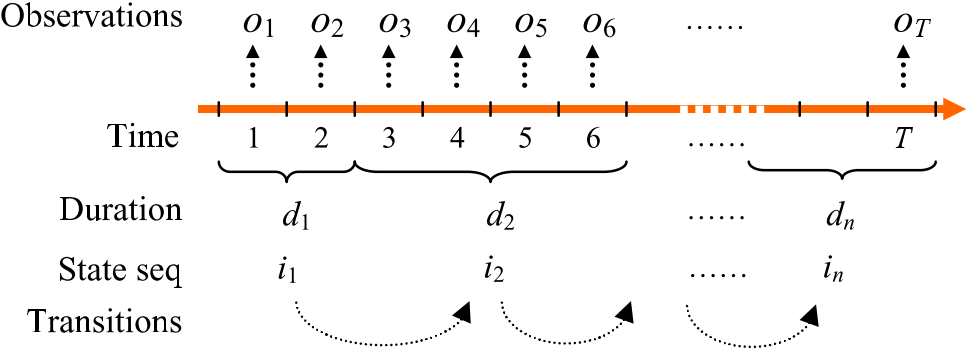
\includegraphics[width=.60\linewidth]{hsmm_representation.png}
                    \caption{Yu, 2010}
                \end{figure}
                \vskip-2cm
                \textbf{Assume :}
                %\vskip0.1cm
                \begin{itemize}
                    \item[\bullet] the set of observable values $\mathcal{V} = \{ v_1,..., v_K\}$
                    where $O_t \in \mathcal{V}$ is the state at time $t$. $O_{1:T}$ is the observed state sequence,
                    $o_{1:T}$ a realization
                    \item[\bullet] the set of hidden states $\mathcal{S}=\{1,...,M\}$
                    where $S_t \in \mathcal{S}$ is the state at time $t$. $S_{1:T}$ is the hidden state sequence,
                    $s_{1:T}$ a realization
                    \item[\bullet] the state duration $d \in \mathcal{D}=\{1,...,D\}$
                \end{itemize}

                \vskip0.5cm
                \textbf{Model :} Explicit-duration HMM, assuming process starts at $t=1$ and ends at $T$
                \vskip0cm
                \begin{itemize}
                    \item[\bullet] the initial distribution :
                    $$\pi_{j,d} \equiv P(S_{1:d} = j, S_{d+1} \neq j)$$
                    \item[\bullet] the state transition probability from $(i,d')$ to $(j,d)$, $i \neq j$ :
                    $$a_{(i,d')(j,d)}=a_{ij}p_j(d)$$
                    $$a_{ij} \equiv P(S_{t+1} = j | S_t = i)$$
                    $$p_j(d) \equiv P(S_{t+1:t+d} = j, S_{t+d+1} \neq j | S_t \neq j)$$
                    \item[\bullet] the emission probability :
                    $$b_{j,d}(o_{t+1}) \equiv P(o_{t+1:t+d} | S_{t+1:t+d} = j)$$
                    \item[\bullet] the parameters of the model : $\lambda \equiv \{a_{(i,d')(j,d)},b_{j,d}(v_{k_1:k_d}), \pi_{i,d}\}$
                \end{itemize}

            \end{block}
          }
        \end{minipage}
      \end{beamercolorbox}
    \end{column}
    % ---------------------------------------------------------%
    % end the column

    % ---------------------------------------------------------%
    % Set up a column
    \begin{column}{.50\textwidth}
      \begin{beamercolorbox}[center,wd=\textwidth]{postercolumn}
        \begin{minipage}[T]{.98\textwidth} % tweaks the width, makes a new \textwidth
          \parbox[t][\columnheight]{\textwidth}{ % must be some better way to set the the height, width and textwidth simultaneously
            % Since all columns are the same length, it is all nice and tidy.  You have to get the height empirically
            % ---------------------------------------------------------%
            % fill each column with content
            \begin{block}{Inference \& Learning in HSMM}
                \textbf{Inference :}
                %\vskip0.5cm
                \textbf{Forward-Backward} algorithm to maintain tractability in inference problems.
                (e.g. expectations such as $P(o_1, ..., o_T | \lambda)$.)\\
                Interestingly, the joint MAP estimate of the state that ends at time $t$ and the duration of this state,
                observing a specific sequence $o_1, ..., o_T$ i.e.
                { $$(\hat s_t, \hat d_t) = \underset{(j,d)}{\mathrm{arg~max}} P(S_{t-d} \neq j, S_{t-d+1:t} = j, S_{t+1} \neq j, o_{1:t} | \lambda)$$}
                can be estimated via MLE using \textbf{Viterbi} algorithms.

                \vskip1cm
                \textbf{Learning :}
                %\vskip0.5cm
                MLE of $\lambda$ via the iterative \textbf{Expectation-Maximization} algorithm :\\
                E-step : find the posterior distribution {\small $P(S_1, ..., S_T | O_1, ..., O_T, \lambda^{old})$}\\
                M-step : maximize le log-likelihood with respect to $\lambda$
            \end{block}

            \vfill
            \begin{block}{Application to eye-movement data}
                \begin{itemize}
                    \item[\bullet] The time index $t$ corresponds to a fixation.
                    \item[\bullet] $\mathcal{V} = \{\text{Forward+, Forward, Refixation, Backward, Backward+}\}$
                    \item[\bullet] $M = 5$ reading strategies estimated by maximizing BIC criterion
                \end{itemize}
                \begin{figure}[h]
                    \centering
                    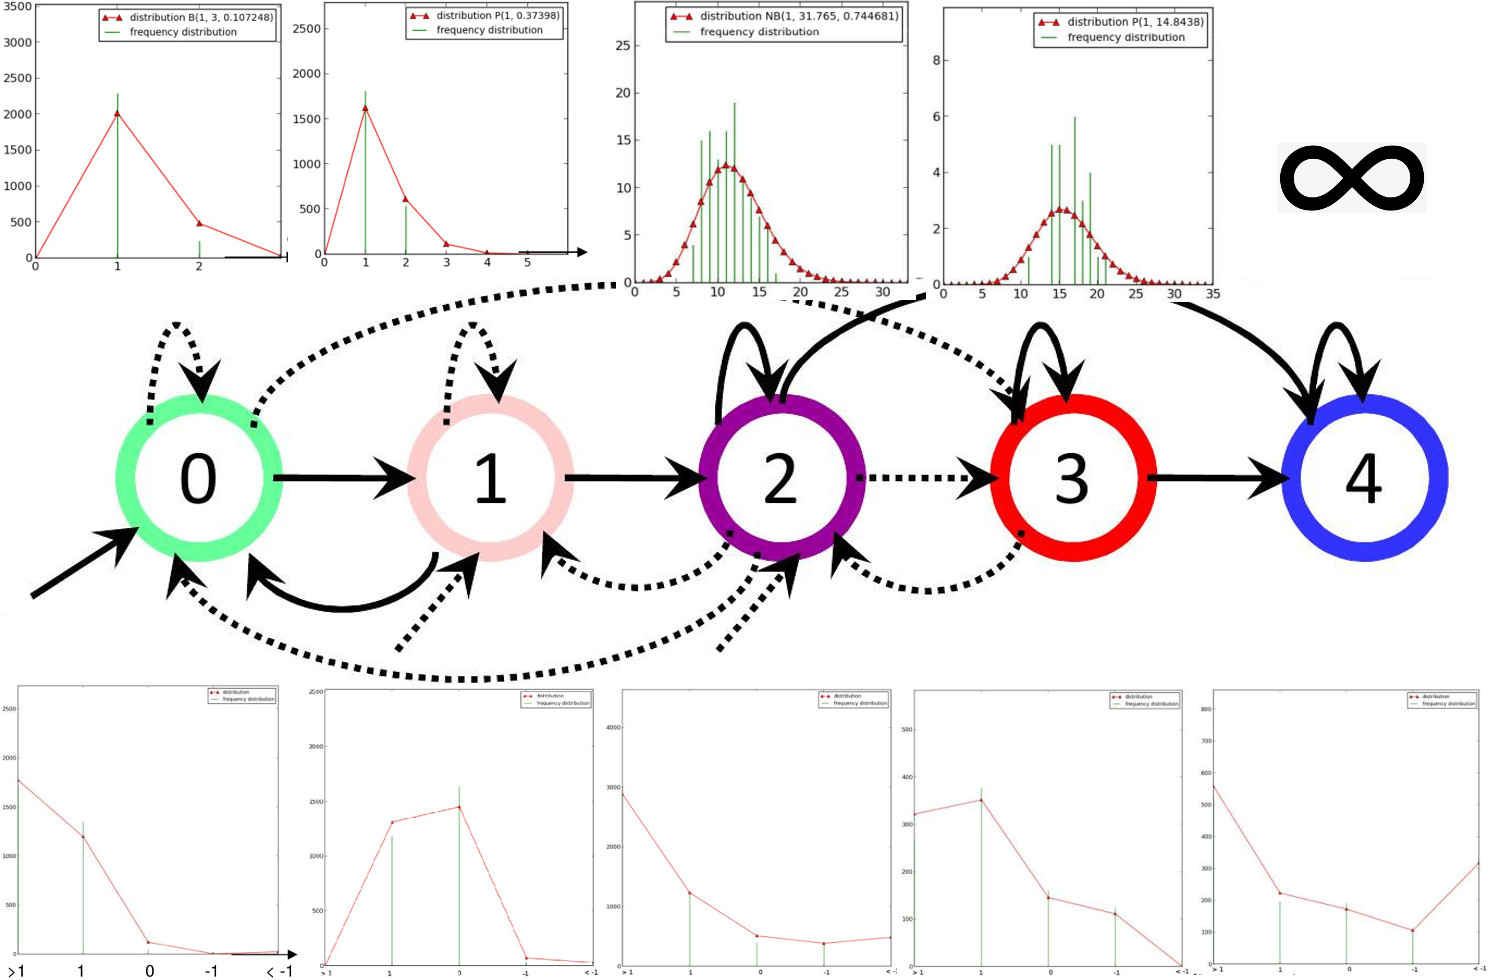
\includegraphics[width=29.75cm]{hsmm.jpg}
                    \caption{HSMM. top bar charts : sojourn time distributions.
                    automaton : transition probabilities.
                    bottom bar charts : emission probabilities.}
                \end{figure}
                4 interpretable strategies uncovered and validated according to reading theory and by analyzing coviariates
                (fixation duration, saccade amplitude, proximity of the word fixated to the goal) :
                {\small$$\mathcal{S}=\{\text{0-1 : Normal reading, 2 : Speed reading, 3 : Careful reading, 4 : Confirmation}\}$$}
                \begin{minipage}{0.47\textwidth}
                    \begin{figure}[h]
                        \centering
                        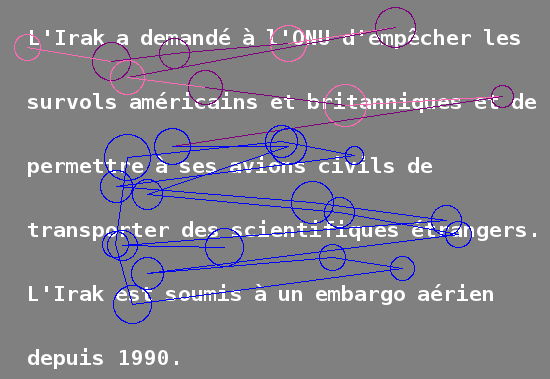
\includegraphics[width=18cm]{scanpath-careful-reader-subj-8-text-14.png}
                    \end{figure}
                \end{minipage} \hfill
                \begin{minipage}{0.47\textwidth}
                    \begin{figure}[h]
                        \centering
                        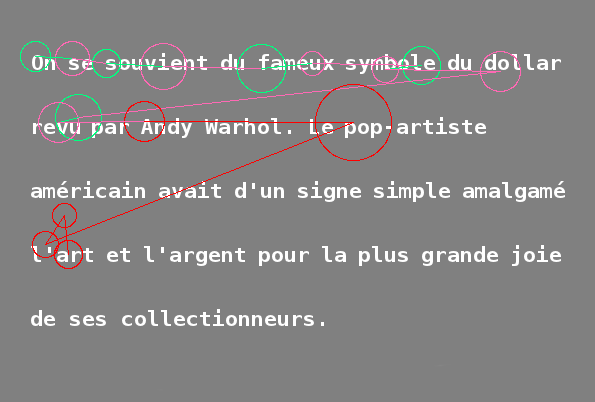
\includegraphics[width=18cm]{scanpath-trained-reader-subj-13-text-5.png}
                    \end{figure}
                \end{minipage}
                \vskip 0.5cm
                \textbf{Issues adressed :}
                \begin{itemize}
                    \item[\bullet] Text variability : evolution of text relativeness to the topic
                    \item[\bullet] Individual variability : trained vs. careful readers
                \end{itemize}
            \end{block}

            %\vfill
            %\begin{block}{EEG data}
            %\end{block}

            \vfill
            \begin{block}{Perspectives}
                \vskip0.2cm
                \begin{minipage}{0.67\textwidth}
                    \begin{itemize}
                        \item[\bullet] Since there is a lot of variability in the text and individuals,
                        propose a clustering approach to reduce variability of the model (mixtures of HSMM)
                        \item[\bullet] Couple eye-movement and EEG data into a single HSMM framework handling signals overlap
                    \end{itemize}
                \end{minipage}
                \begin{minipage}{0.30\textwidth}
                    \begin{figure}[h]
                        \centering
                        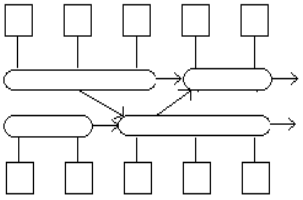
\includegraphics[heigth=10cm]{chsmm_representation.png}
                        \caption{Natarajan, 2007}
                    \end{figure}
                \end{minipage}


            \end{block}

            \vfill
            \begin{block}{References}
                \begin{enumerate}
                    {\footnotesize
                    \item Frey, A. et al.
                    Decision-making in information seeking on texts: an eye-fixation-related potentials investigation.
                    \textit{Frontiers in systems neuroscience} 7 (8): 1-22 (2013)

                    \item Natarajan P. et al.
                    Coupled Hidden Semi Markov Models for Activity Recognition.
                    \textit{Motion and video computing} (2007)

                    \item Simola, J. et al.
                    Using hidden Markov model to uncover processing states from eye movements in information search tasks
                    \textit{Cognitive Systems Research} 9 (4): 237-251 (2008)

                    \item Yu, S-Z.
                    Hidden semi-Markov models.
                    \textit{Artificial Intelligence} 174 (2): 215-143 (2010)
                    }
                \end{enumerate}
            \end{block}
          }
          % ---------------------------------------------------------%
          % end the column
        \end{minipage}
      \end{beamercolorbox}
    \end{column}
    % ---------------------------------------------------------%
    % end the column
  \end{columns}
  \vskip1ex
  %\tiny\hfill\textcolor{ta2gray}{Created with \LaTeX \texttt{beamerposter}  \url{http://www-i6.informatik.rwth-aachen.de/~dreuw/latexbeamerposter.php}}
  %\tiny\hfill{Created with \LaTeX \texttt{beamerposter}  \url{http://www-i6.informatik.rwth-aachen.de/~dreuw/latexbeamerposter.php} \hskip1em}
\end{frame}
\end{document}


%%%%%%%%%%%%%%%%%%%%%%%%%%%%%%%%%%%%%%%%%%%%%%%%%%%%%%%%%%%%%%%%%%%%%%%%%%%%%%%%%%%%%%%%%%%%%%%%%%%%
%%% Local Variables:
%%% mode: latex
%%% TeX-PDF-mode: t
%%% End:
